\chapter{Appendix}

\section*{Appendix 1: Indvidual Stock Results}

\newpage
\newcolumntype{P}[1]{>{\centering\arraybackslash}p{#1}}
\begin{landscape}
\begin{longtable}{P{1.7cm}P{1.7cm}P{1.7cm}P{1.7cm}P{1.7cm}P{1.7cm}P{1.7cm}P{1.7cm}P{1.7cm}P{1.7cm}} 
\caption{Forecast Stocks}
\label{Forecast Stocks}\\
\hline
\textbf{Ticker} & \textbf{IV }$\boldsymbol{\%}$ & $\boldsymbol{r_{economic}}$ & $\boldsymbol{\sigma_{economic}}$ & \textbf{Sign Ratio} &  $\boldsymbol{r_{sign}}$ & $\boldsymbol{\sigma_{sign}}$ & $\boldsymbol{\alpha}$ & $\boldsymbol{\bar\epsilon_{forecast}}$ & $\boldsymbol{\sigma_{forecast}}$  \\
\hline
\endfirsthead
\multicolumn{10}{c}%
{\tablename\ \thetable\ -- \textit{Continued from previous page}} \\
\hline
\textbf{Ticker} &  \textbf{IV }$\boldsymbol{\%}$ & $\boldsymbol{r_{economic}}$&  $\boldsymbol{\sigma_{economic}}$  & \textbf{Sign Ratio} &  $\boldsymbol{r_{sign}}$ &  $\boldsymbol{\sigma_{sign}}$ &  $\boldsymbol{\alpha}$ & $\boldsymbol{\bar\epsilon_{forecast}}$ & $\boldsymbol{\sigma_{forecast}}$  \\
\hline
\endhead
\hline \multicolumn{10}{r}{\textit{Continued on next page}} \\
\endfoot
\hline
\endlastfoot
\input{Input/ForecastsStocks.txt}
\end{longtable}
\end{landscape}

IV er gjennomsnittlig for hele perioden


\section*{Appendix 2: Bucket economic return versus sign return}
\begin{figure}[h]
    \centering
    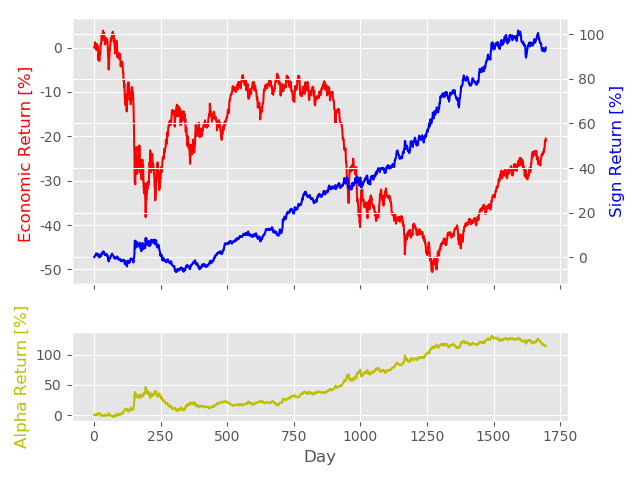
\includegraphics[scale = 0.5]{Plot/BucketNumber1ReturnPlot.png}
    \caption{Regression: IV to forecasting error}
    \label{visualization}
\end{figure}

\begin{figure}[h]
    \centering
    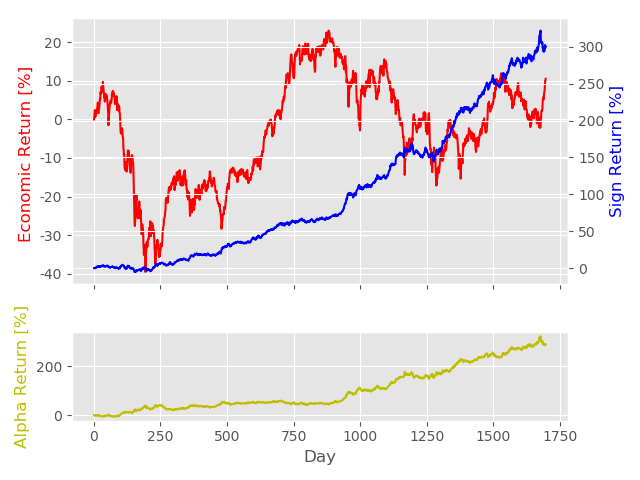
\includegraphics[scale = 0.5]{Plot/BucketNumber2ReturnPlot.png}
    \caption{Regression: IV to forecasting error}
    \label{visualization}
\end{figure}

\begin{figure}[h]
    \centering
    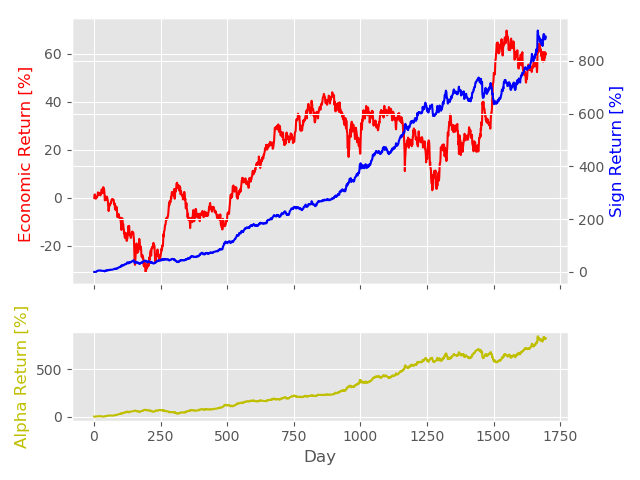
\includegraphics[scale = 0.5]{Plot/BucketNumber3ReturnPlot.png}
    \caption{Regression: IV to forecasting error}
    \label{visualization}
\end{figure}

\begin{figure}[h]
    \centering
    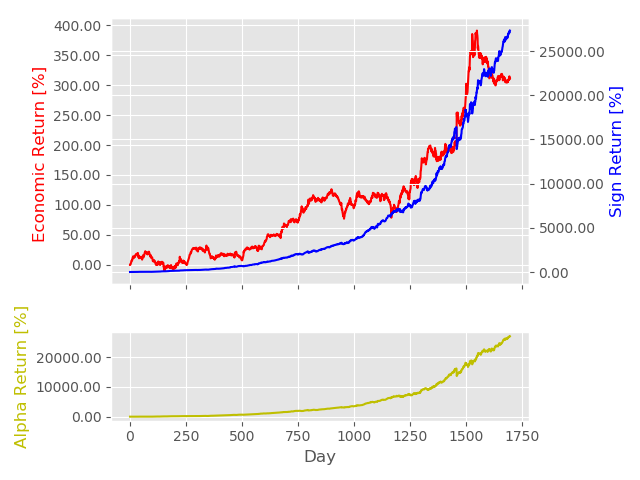
\includegraphics[scale = 0.5]{Plot/BucketNumber4ReturnPlot.png}
    \caption{Regression: IV to forecasting error}
    \label{visualization}
\end{figure}